\section{MANEUVER PERFORMANCE}

\begin{whitebox}{}
    \begin{tabularx}{\columnwidth}{lclclc}
        $a_n$ & $\unit{m.s^{-2}}$ & Centripetal acceleration\\
        $r$ & $\unit{m}$ & Turn radius\\
        $\Psi$ & $\unit{rad}$ & Turn angle\\
        $\dot{\Psi}$ & $\unit{rad.s^{-1}}$ & Turn rate\\
        $\dot{\phi}$ & $\unit{rad}$ & Bank angle\\
        $n$ & $-$ & Load factor
    \end{tabularx}
\end{whitebox}

\begin{whitebox}{\textbf{STATIONARY LEVEL TURN}}
    \blue{Conditions}
    \begin{itemize}
        \item $V=$ const.
        \item $\gamma=0$ i.e. $h=$ const.
        \item $r=$ const.
    \end{itemize}

    \centering
    \resizebox{0.5\linewidth}{!}{
        \includegraphics[
        page = {8},
        trim = {3.0cm, 8.7cm, 16.5cm, 2.8cm}, % left, bottom, right, top
        clip
        ]{Lecture04.pdf}
    }
    \resizebox{0.7\linewidth}{!}{
        \includegraphics[
        page = {8},
        trim = {2.0cm, 2.5cm, 15.0cm, 11.0cm}, % left, bottom, right, top
        clip
        ]{Lecture04.pdf}
    }
    \begin{highlightbox}{}
        \begin{align}
            \label{eq:stat_turn_thrust}
            &T=D\\
            \label{eq:stat_turn_vertical}
            &L\cos\phi=mg\\
            \label{eq:stat_turn_normal}
            &L\sin\phi=ma_n
        \end{align}
    \end{highlightbox}

    \begin{highlightbox}{CENTRIPETAL ACCELERATION}
        \begin{align}
            \label{eq:stat_turn_centrip}
            &a_n=\frac{V^2}{r}=V\frac{V}{r}=V\dot{\Psi}
        \end{align}
    \end{highlightbox}

    \begin{highlightbox}{LOAD FACTOR}
        \begin{align}
            \label{eq:stat_turn_load}
            &n=\frac{L}{mg}
        \end{align}
    \end{highlightbox}

    \mathbox{
        \dot{\Psi}=\frac{V}{r}
    }
    \mathbox{
        \dot{\Psi}=\frac{g\tan\phi}{V}
    }
    \mathbox{
        r=\frac{V^2}{g\sqrt{n^2-1}}
    }
    \mathbox{
        \dot{\Psi}=\frac{g\sqrt{n^2-1}}{V}
    }
    \begin{whitebox}{\textbf{PERFORMANCE}}
        \resizebox{1.0\linewidth}{!}{
            \includegraphics[
            page = {12},
            trim = {3.0cm, 3.0cm, 4.0cm, 3.0cm}, % left, bottom, right, top
            clip
            ]{Lecture04.pdf}
        }
        \resizebox{1.0\linewidth}{!}{
            \includegraphics[
            page = {16},
            trim = {3.0cm, 3.0cm, 4.0cm, 3.0cm}, % left, bottom, right, top
            clip
            ]{Lecture04.pdf}
        }
    \end{whitebox}
\end{whitebox}

